\subsubsection{RFID}
\label{subsubsec:Inbetriebnahme_RFID}

Beim RFID-Leser handelt es sich wie in Kapitel \ref{subsubsec:RFID} beschrieben um das MFRC522 Evaluierungsboard (Breakout-Board). Dieses Kommuniziert über SPI mit einem gewünschten Controller. Die Pinbelegung dazu ist in Abbildung \ref{fig:MFRC522} zu sehen. Der grosse Vorteil dieses Evaluierungsboard ist es, dass es dazu eine Arduino Library gibt mit vielen Beispielen. Wie schon in Kapitel \ref{sec:Printaufbau} beschrieben, wurde das ESP schlussendlich nicht an den Mikrocontroller angeschlossen, sondern an das ESP32, welches dann wiederum mit dem Mikrocontroller kommuniziert. Um den Leser in Betrieb nehmen zu können, wurde dieser wie folgt angeschlossen:


\begin{itemize}
\item Vcc: An 3.3V vom ESP32
\item GND: An GND vom ESP32
\item SDA: An IO5 vom ESP32
\item SCK: An IO18 vom ESP32
\item MISO: AN IO19 vom ESP32
\item Reset: AN IO22 vom ESP32
\item MOSI: AN IO23 vom ESP32
\end{itemize}

\begin{figure}[h!]
\center
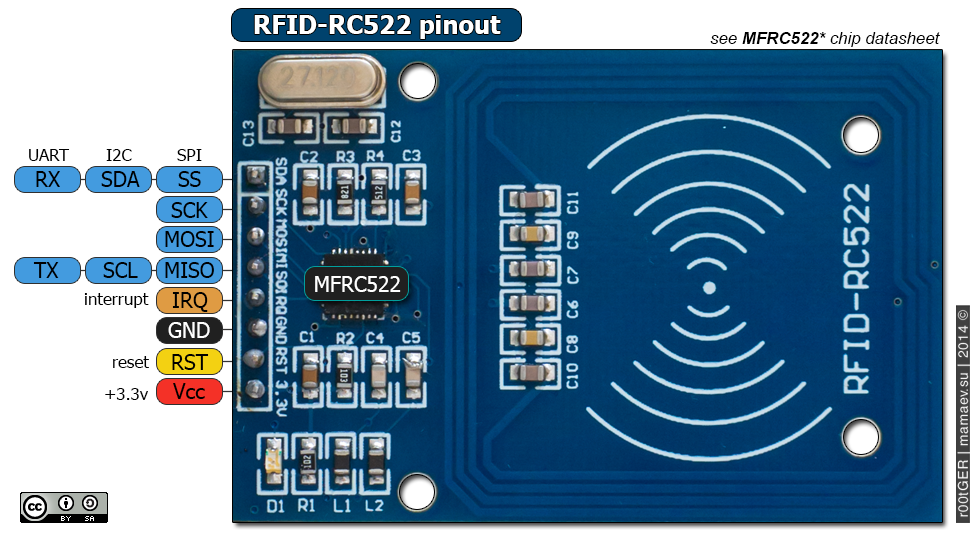
\includegraphics[width = 0.45\textwidth]{graphics/MFRC522}
\caption{Anschauungsbild MFRC522 Evaluierungsboard \cite{nxp_bv_2010_antenna_2010}}
\label{fig:MFRC522}
\end{figure}

Diese Pinbelegung ist von der Arduino-Library gegeben und wird auch so bei der Cocktailmaschine eingesetzt, da es keinen Grund gibt diese direkt in der Library zu ändern. Lediglich die beiden Pin's \flqq SDA\frqq~und \flqq Reset\frqq~können flexibel festgelegt werden.

Um das Lesegerät in Betrieb nehmen zu können, wurden nach dem Anschliessen des ESP32 an den Computer folgende Schritte unternommen: 

\begin{enumerate}
\item Einbinden der MFRC522 Library unter: \textcolor{blue}{Werkzeuge \textrightarrow Bibliotheken verwalten} \newline
\item Öffnen des Beispiels DunmInfo unter: \textcolor{blue}{Datei \textrightarrow Beispiele \textrightarrow MFRC522 \textrightarrow DumpInfo} \newline
\item Einstellen des Reset und des SDA (SS) Pin's in den defines des Codes\newline
\item Einbinden des ESP32-Boards unter: \textcolor{blue}{Werkzeuge \textrightarrow Board \textrightarrow Boardverwalter \textrightarrow esp32} \newline
\item Einstellen des verwendeten Boards unter: \textcolor{blue}{Werkzeuge \textrightarrow Board \textrightarrow ESP32 Arduino \textrightarrow ESP32 Dev Module} \newline
\item Einstellen des richtigen COM-Ports unter: \textcolor{blue}{Werkzeuge \textrightarrow Port} (Kann im Geräte-Manager des Computers nachgeschaut werden) \newline
\item Upload des Pogrammes mittels Upload-Button \newline
\item Öffnen des Serial Monitors unter: \textcolor{blue}{Werkzeuge \textrightarrow  Serieller Monitor} \newline
\end{enumerate}

Nun konnten die verschiedenen RFID-Tag's eingelesen werden und  die gelesenen Informationen wurden am seriellen Monitor ausgegeben. \cite{pcbreflux_esp32_2017}




